\section{Продвинутые подходы автоматизации тестирования} 

До настоящего момента под <<автоматизацией>> понималась автоматизация выполнения тестов. Продвинутые подходы к автоматизации тестирования расширяют понятие атоматизиции. Они исключают человеческий фактор в процессе тестирования. Это означает отсутсвие необходимости разрабатывать тестовые сценарии. Компьютер сделает это за человека. Иногда такие подходы называются тестированием с помощью искусственного интелекта.

\subsection{Статическое тестирование} 

Статическое тестирование (статический анализ)~--- автоматизированный процесс ревизии кода без его исполнения. Статическое тестирование позволяет быстро найти ошибки низкой и средней сложности (использование неактуальной библиотеки, обращение к пустому указателю и т.~д.). Распространенные инструменты статического анализа: \textit{PMD, Checkstyle, Checkmarx}.

Классический подход к статическому анализу заключается в проверке исходного кода системы на потенциальные структурные или стилистические уязвимости. Анализатор состоит из парсера и набора правил. Существуют две техники статического анализа:


\begin{enumerate}
	\item Сопоставление с образцом с помощью регулярных выражений.
	\item Синтаксический анализ абстрактного ситаксического дерева.
\end{enumerate}


\subsubsection{Сопоставление с образцом}

Сопоставление с образцом~--- проверка кода, входе которой происходит поиск соответствия заданному ранее образцу. Образец задается с помощью \textbf{регулярного выражения}. Регулярное выражение~--- последовательность символов, представляющая образец.

Недостатком сопоставления с образцом является отсутствие контекта исполнения. Другими словами, сопоставление с образцом не учитывает семантику программы. Например, задав регулярное выражение \texttt{$\textbackslash$s*System.out.println\textbackslash(.*\textbackslash);} сопоставление с образцом определит 3 строки в листинге~1.17. Из чего можно сделать вывод, что программа напечатает 3 раза некоторое сообщение. Однако, программа не напечатает ни одного сообщения. 

\begin{ListingEnv}[!h]% настройки floating аналогичны окружению figure
	\captiondelim{ } % разделитель идентификатора с номером от наименования
	\caption{Пример неучитанной семантики}
	% окружение учитывает пробелы и табуляции и применяет их в сответсвии с настройками
	\begin{lstlisting}[language={Java}]
boolean DEBUG = false;

if (DEBUG){
	System.out.println("Debug line 1");
	System.out.println("Debug line 2");
	System.out.println("Debug line 3");
}
	\end{lstlisting}
\end{ListingEnv}%


\subsubsection{Синтаксический анализ}

Более продвинутый способ анализа кода~--- синтаксический анализ. В ходе синтаксического анализа текст программы разбивается на поток символов, символы пребразубтся в токены, а из токенов составляется \textit{дерево разбора}. Дераво разбора представляет собой синтаксическое дерево конкретной версии кода. В синтаксическом анализе используется \textit{абстрактое синтаксическое дерево}~--- дерево разбора без синтаксических деталей (точки с запятой, скобки). Пример абстрактного синтаксического дерева кода из листинга~1.17 представлен на рис.~\ref{img:ast}

\begin{figure}[ht]
	\centering
	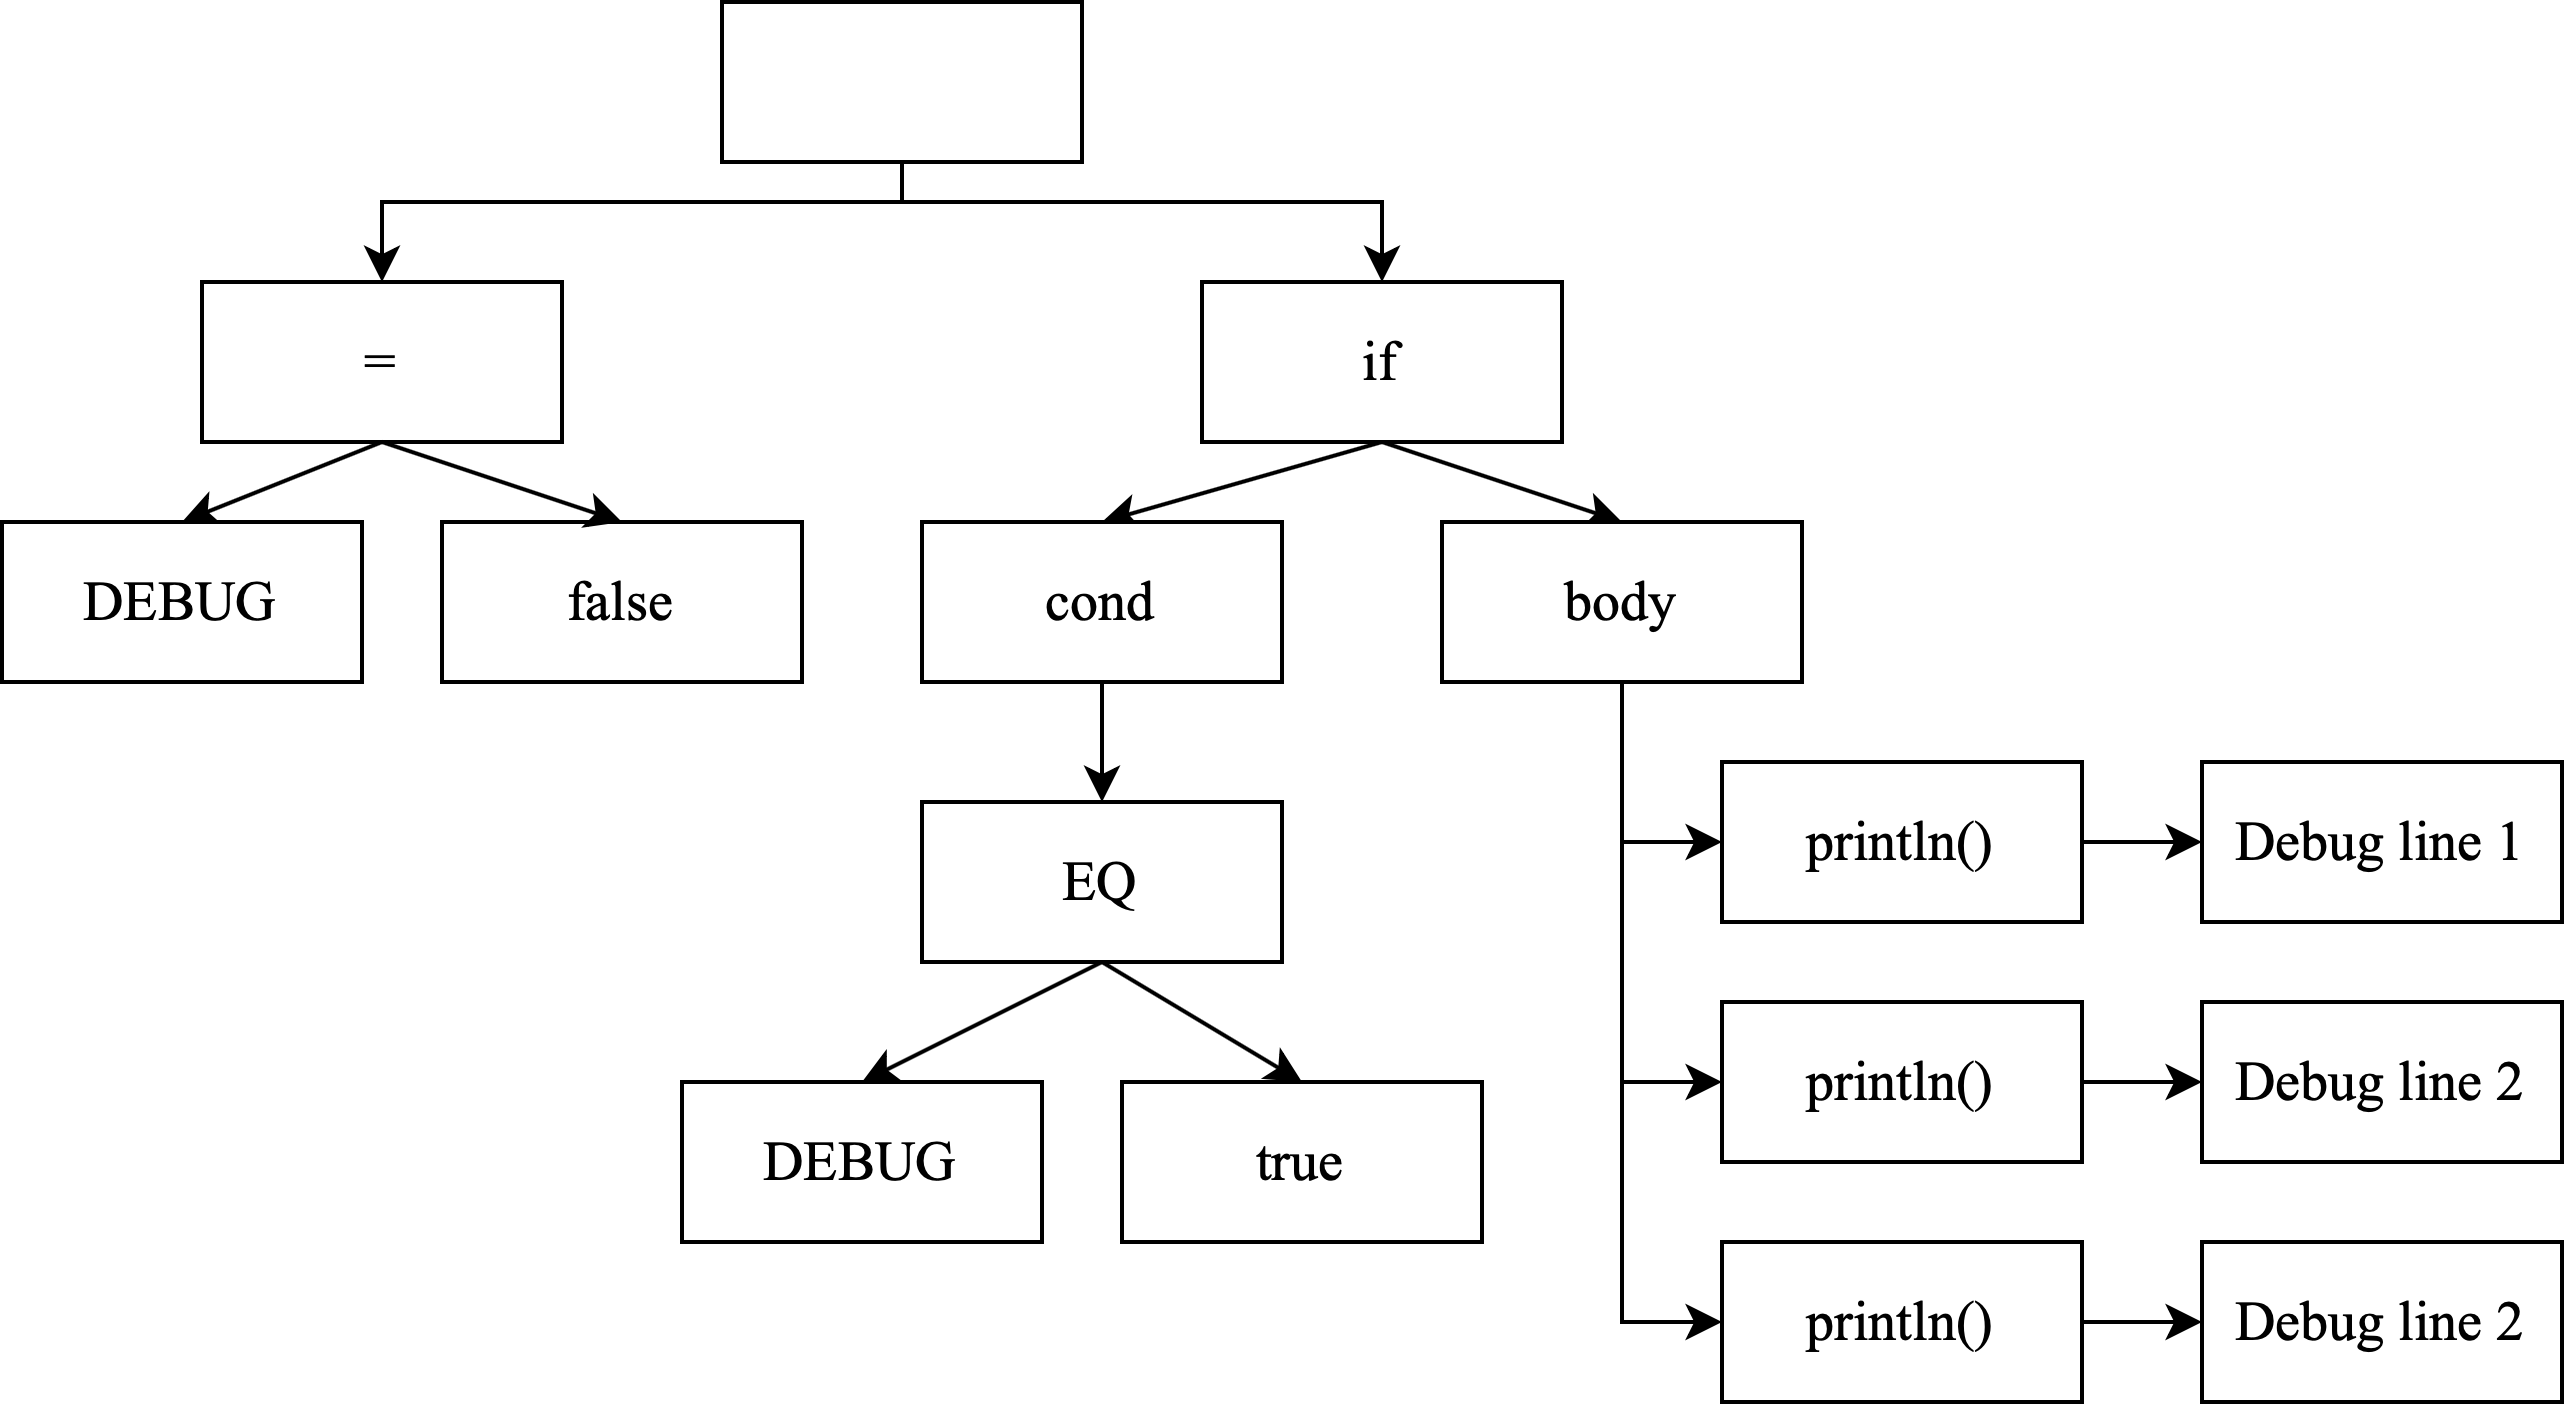
\includegraphics [scale=0.9] {AST_TR}
	\caption{Абстрактное синтаксическое дерево}
	\label{img:ast}
\end{figure}


Статический анализатор, использующий ситаксический анализ, принимает на вход абстрактное синтаксическое дерево и набор правил. Анализатор сообщает о найденных несоответствиях в коде.


\subsection{Мутационное тестирование} 
  
При рассмотрении структурного тестирования были описанны различные критерии покрытия кода. Эти критерии нужны для того, чтобы измерить объем кода, выполненного в ходе тестирования. К сожалению, таких критериев может быть не достаточно для оценки качества тестов. Например, тест может достигать 100~\% покрытия кода, но в то же время не содержать проверок (assertions). То есть тест запускает код, но не тестирует результат его исполнения. Мутационное тестирование решает эту проблему.
 
Критерий, который отражает насколько эффективнен тест, называется критерием \textit{способности определения ошибок(fault detection capability)}. Этот критерий составляет основу \textbf{мутационного тестирования}. В процессе мутационного тестироания в код программы добавляются (искуственно) ошибки. После чего запускается набор тестов и проверяется, смогли ли тесты найти ошибку. Цель мутационного тестирования~--- повышение качества тестирующего кода. Чем больше ошибок тест может найти, тем выше его эффективность.

Терминология в мутационном тестировании:

\begin{itemize}
	\item \textbf{Мутант.} Для данной программы \textit{P}, мутантом называется программа \textit{P'}, полученная из программы \textit{P} путём \textit{синтаксической трансформации}. Мутант считается убитым, если он не проходит хотя бы один тест.
	\item \textbf{Синтаксическая трансформация.} Небольшое изменение кода, при котором код все еще компилируется.
	\item \textbf{Изменение.} Имитация типичной человеческой ошибки. 
\end{itemize}

Для атоматизации мутационного тестирования необходимо определить \textbf{мутационный оператор}. Мутационный оператор~--- граматическое правило, которое может быть использования для создания синтаксической трансформации. Например, замена знака \(+\) на 
\(-\) в арифметических выражениях. Распространенные мутационные операторы:

\begin{itemize}
	\item \textbf{Оператор арифметической замены.} Замена арифметечиского оператора на другой. Арифметические операторы: \texttt{+, -, *, /,\%}.
	\item \textbf{Оператор замены сравнений.} Замена операторов \texttt{<=, >=, !=, ==, >, <}.
	\item \textbf{Оператор логической замены.} Замена операторов \texttt{\&\&, ||, \&, |, !, \^}.
	\item \textbf{Оператор замены присваения.} Замена операторов \texttt{=, +=, -=, /=}.
	\item \textbf{Оператор замены скалярных переменных.}  Замена одной переменной на другую.
\end{itemize}

Помимо описанных выше метационных оперторов, существуют операторы, ориентированные на особонности языка. Например, оператор замены модификоторов видимости, переопределение метода и т.~д.

Для оценки качества тестового сценария с помощью мутационного анализа используется \textit{критерий устойчивости к мутациям}.

\[ \text{критерий устойчивости к мутациям} = \frac{\text{количество убитых мутантов}}{\text{общее количество мутантов}}  \]

Чем больше мутантов убивает тест, тем выше его критерий устойчивости к мутациям. Соответсвенно, этот тест найдет больше реальных ошибок программистов. 

Недостатком мутационного тестирования является время исполнения. На проектах средней сложности (300 файлов) мутационное тестирование занимает около 10 минут~[9].

В языке Java для мутационного тестирования используется инструмент PIT~[10].

\subsection{Генерация входных данных} 
 
 \fixme{TBD}
 

\subsection{Тестирование на основе анализа кода} 
 
 \fixme{TBD}
 
